\section{Experiments}

\subsection{Proposed Modifications}
We investigated various aspects of the methodology, including:
\begin{enumerate}
    \item The relevance of dimensionality reduction applied to features before training the neural networks.
    \item The rationale for opting for a graph-based classification approach rather than a simple dense network operating on the vectorized feature vectors.
\end{enumerate}
As a result, we explored different techniques for dimensionality reduction and various classification models. We run the following experiments to address these questions.

Initially, we trained the models using the original features without any dimensionality reduction (1). Subsequently, we trained them with a reduced number of features achieved through recursive feature elimination (2), mirroring the approach detailed in the referenced paper. Finally, we applied an autoencoder to reduce feature dimensionality (3).

We implemented three distinct models:
\begin{enumerate}
    \item A simple Dense Neural Network consisting of linear layers and ReLU activations.
    \item A Graph Convolutional Network (GCN) as outlined in \cite{kipf_semi-supervised_2017}, incorporating the \textit{renormalization trick}.
    \item A neural network utilizing Chebyshev polynomials with an order of $K=3$, in accordance with the methodology presented in the referenced paper \cite{Parisot17}.
\end{enumerate}


\subsection{Dimensionality reduction by Recursive Feature Selection with a Ridge classifier}

A Ridge classifier is a standard linear classifier with an added regularization term known as the Ridge (L2) penalty.

The optimization problem of the ridge classifier is to find the coefficients $\beta$ that minimize the following objective function:
$$
\min_{\beta} \norm{y - X\beta}_2^2 + \alpha \norm{\beta}_2^2
$$
where $X$ is the design matrix, here the vectorized connectivity matrix, $y$ is the corresponding target value, $\alpha$ is the regularization parameter, and $\norm{.}_2$ denotes the Euclidean norm. The ridge classifier converts the targets values into $\{-1, 1\}$ and then treats the problem as a regression task. The predicted class corresponds to the sign of the regressor's prediction, which is
$$
\hat{y} = sign(X\hat{\beta})
$$
where $sign$ is a function that return $1$ if the input is positive, $-1$ if the input is negative, and $0$ if the input is zero.
% The Ridge penalty term, $\alpha \lVert w \rVert_2^2$, penalizes large values of the weights, encouraging a more generalizable model and helping to mitigate overfitting.

The recursive feature elimination (RFE) is employed to iteratively select features by progessively considering smaller sets of features. Initially, the estimator is trained on the complete set of features, and the importance of each feature $i$ is determined by evaluating the weights assigned in the Ridge esimator $\hat{\beta}_i$. Subsequently, the least important features are pruned from current set and this process is repeated recursively repeated on the pruned set until the desired number of selected features is reached.
% \begin{figure*}[t!]
%     \centering
%     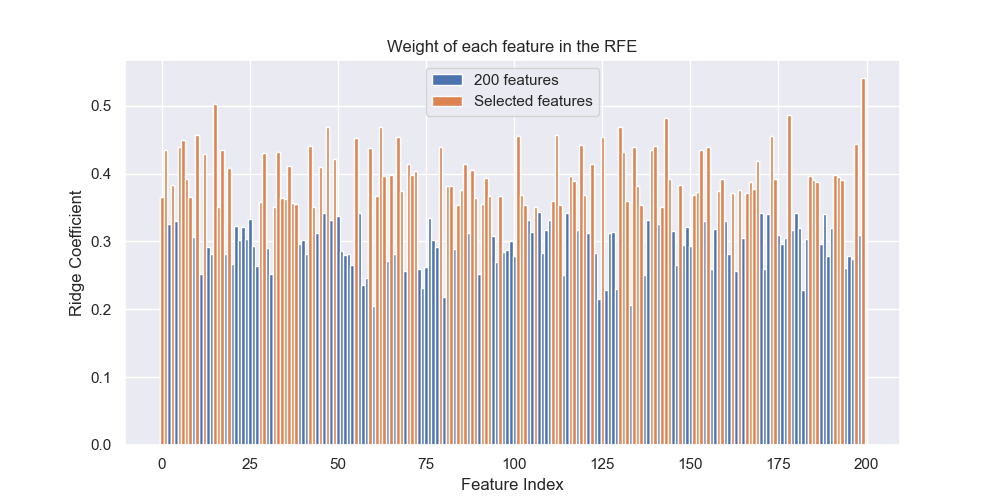
\includegraphics[width=0.8\textwidth]{figures/rfe.png}
%     \caption{Relative importance of features for recursive elimination}
%     \label{fig:rfe}
%     \Description{}
% \end{figure*}

\subsection{Dimensionality reduction by Autoencoder}


